\documentclass[10pt,aspectratio=169]{beamer}

\usetheme{Madrid}
\usecolortheme{default}

\usepackage{booktabs}
\usepackage{amsmath}
\usepackage{graphicx}
\usepackage{hyperref}
\usepackage{tikz}

\title[Polymarket Expert-Following Backtest]{An Expert-Following Strategy for Polymarket}
\subtitle{Methodology and Backtest Results}
\author{Shiqi Lei}
\date{\today}

\begin{document}

\begin{frame}
  \titlepage
\end{frame}

\begin{frame}{Executive Summary}
  \begin{itemize}
    \item We test a settlement-only Polymarket strategy that follows historically skilled traders.
    \item Trader expertise is estimated from past settled markets using semantic similarity between market questions.
    \item The current strategy trades only the high-probability ``stable'' bucket: entry price $>0.8$.
    \item The latest full-market-scale backtest covers roughly 3.11 years of trade history.
    \item Final portfolio value is evaluated using total equity, not only cash balance.
  \end{itemize}
\end{frame}

\begin{frame}{Data Sources and Coverage}
  \begin{itemize}
    \item Market metadata is fetched from the Polymarket Gamma API.
    \item Public historical trades are fetched from the Polymarket Data API.
    \item Cached full-market run:
      \begin{itemize}
        \item 299,318 market records.
        \item 1,195,104 normalized trade rows.
        \item 2,993 trade-covered markets.
        \item 2,516 trade-covered markets with available resolution labels.
      \end{itemize}
    \item Local cache is used for markets, trades, and embeddings to make repeated runs practical.
  \end{itemize}
\end{frame}

\begin{frame}{Important Modeling Assumption}
  \begin{block}{Settlement-only PnL}
    We do not model mid-market exits, stop-losses, or selling before resolution.
    Every position is evaluated by final settlement or by mark-to-last-known trade price if still open.
  \end{block}

  \vspace{0.3cm}
  \begin{itemize}
    \item This differs from stock-style backtests.
    \item It matches the intended research question: buy a prediction market outcome and hold until final resolution.
    \item Reported \texttt{total\_equity} is preferred over \texttt{final\_balance}, because open positions may lock cash.
  \end{itemize}
\end{frame}

\begin{frame}{Anti-Leakage Design}
  \begin{itemize}
    \item The event stream is processed chronologically.
    \item At time $t$, trader skill uses only markets settled no later than $t$.
    \item Current market resolution is never used to generate current signals.
    \item A signal is executed only after a configurable delay.
    \item Time-to-resolution filters are computed using market metadata available at entry time.
  \end{itemize}
\end{frame}

\begin{frame}{Trader Market Score}
  For trader $u$ in settled market $m$:

  \[
    \text{score}_{u,m}
    =
    \operatorname{clip}
    \left(
      \frac{\text{PnL}_{u,m}}{\text{notional}_{u,m}},
      -1,
      1
    \right)
  \]

  \vspace{0.2cm}
  where:
  \begin{itemize}
    \item \texttt{notional} is absolute traded dollar volume.
    \item \texttt{PnL} is computed from cash flows plus final settlement payout.
    \item Scores are clipped to reduce extreme unit-return outliers.
  \end{itemize}
\end{frame}

\begin{frame}{Semantic Similarity Between Markets}
  Each market question is embedded into a vector:

  \[
    e_m = \operatorname{Embed}(\text{question}_m)
  \]

  Similarity is cosine similarity:

  \[
    s(m, n) = \max \left(0, \cos(e_m, e_n)\right)
  \]

  \vspace{0.2cm}
  Current implementation supports:
  \begin{itemize}
    \item \texttt{sentence\_transformers}: currently \texttt{BAAI/bge-large-en-v1.5}.
    \item \texttt{hashing}: faster fallback for parameter sweeps.
  \end{itemize}
\end{frame}

\begin{frame}{Trader Skill on a New Market}
  For trader $u$ and target market $q$ at time $t$:

  \[
    \widehat{\text{skill}}_{u,q,t}
    =
    \frac{
      \sum_{m \in \mathcal{H}_{u,t}}
      s(q,m) \cdot \text{notional}_{u,m} \cdot \text{score}_{u,m}
    }{
      \sum_{m \in \mathcal{H}_{u,t}}
      s(q,m) \cdot \text{notional}_{u,m}
    }
  \]

  \vspace{0.2cm}
  where $\mathcal{H}_{u,t}$ contains only markets already settled by time $t$.

  \vspace{0.2cm}
  A trader is considered skilled in the current flow if:
  \[
    \widehat{\text{skill}}_{u,q,t} \geq \texttt{skill\_threshold}
  \]
\end{frame}

\begin{frame}{Direction Consensus Signal}
  Each skilled trade contributes direction-weighted flow:

  \[
    w_i = \widehat{\text{skill}}_i \cdot \text{volume}_i
  \]

  Direction ratios:

  \[
    R_{\text{YES}} =
    \frac{\sum_{i \in \text{YES}} w_i}
         {\sum_i w_i},
    \quad
    R_{\text{NO}} =
    \frac{\sum_{i \in \text{NO}} w_i}
         {\sum_i w_i}
  \]

  A signal is triggered when:
  \[
    \max(R_{\text{YES}}, R_{\text{NO}})
    \geq
    \texttt{consensus\_threshold}
  \]
\end{frame}

\begin{frame}{Current Strategy Rules}
  Current production-style research configuration:

  \begin{itemize}
    \item Trade only the stable bucket: entry token price $>0.8$.
    \item Lottery bucket is disabled.
    \item Direction must pass expert consensus threshold.
    \item Entry must satisfy:
      \[
        5 < \text{days to resolution} < 40
      \]
    \item Stable bucket position size:
      \[
        \text{notional} = 0.2 \times \text{current cash balance}
      \]
    \item Maximum two entries per market.
  \end{itemize}
\end{frame}

\begin{frame}{Backtest Framework in One Slide}
  \begin{center}
    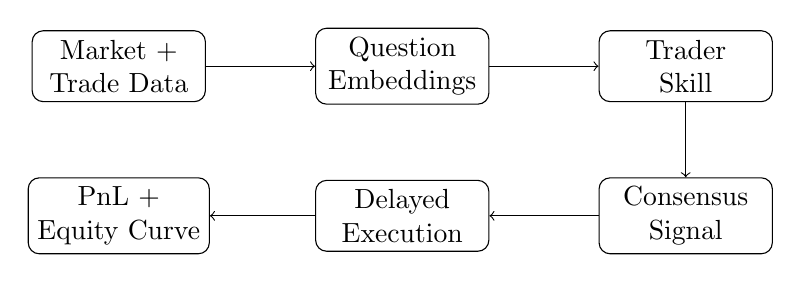
\begin{tikzpicture}[node distance=1.9cm, every node/.style={rectangle, draw, rounded corners, align=center, minimum width=2.2cm, minimum height=0.8cm}]
      \node (data) {Market +\\Trade Data};
      \node (embed) [right of=data, xshift=1.7cm] {Question\\Embeddings};
      \node (skill) [right of=embed, xshift=1.7cm] {Trader\\Skill};
      \node (signal) [below of=skill] {Consensus\\Signal};
      \node (engine) [left of=signal, xshift=-1.7cm] {Delayed\\Execution};
      \node (eval) [left of=engine, xshift=-1.7cm] {PnL +\\Equity Curve};

      \draw[->] (data) -- (embed);
      \draw[->] (embed) -- (skill);
      \draw[->] (skill) -- (signal);
      \draw[->] (signal) -- (engine);
      \draw[->] (engine) -- (eval);
    \end{tikzpicture}
  \end{center}
\end{frame}

\begin{frame}{Backtest Result Snapshot}
  \begin{table}
    \centering
    \begin{tabular}{lr}
      \toprule
      Metric & Value \\
      \midrule
      Trade period & 2023-03-16 to 2026-04-24 \\
      Duration & 1134.95 days / 3.107 years \\
      Markets in universe & 299,318 \\
      Historical trades sampled & 1,195,104 \\
      Unique traders & 330,576 \\
      Strategy trades & 513 \\
      Win rate & 99.03\% \\
      Total realized PnL & 12,541.45 \\
      Average PnL per settled trade & 24.45 \\
      Final total equity & 22,600.15 \\
      Approx. CAGR & 30.00\% \\
      \bottomrule
    \end{tabular}
  \end{table}
\end{frame}

\begin{frame}{Detailed Experimental Results}
  \begin{table}
    \centering
    \begin{tabular}{lr}
      \toprule
      Metric & Value \\
      \midrule
      \texttt{trades} & 513 \\
      \texttt{win\_rate} & 0.990253 \\
      \texttt{total\_pnl} & 12,541.4474 \\
      \texttt{avg\_pnl\_per\_trade} & 24.4473 \\
      \texttt{pnl\_volatility} & 81.3893 \\
      \texttt{final\_balance} & 34.2648 \\
      \texttt{open\_positions} & 27 \\
      \texttt{open\_notional} & 22,507.1826 \\
      \texttt{open\_market\_value} & 22,565.8838 \\
      \texttt{open\_unrealized\_pnl} & 58.7013 \\
      \texttt{total\_equity} & 22,600.1487 \\
      \bottomrule
    \end{tabular}
  \end{table}
\end{frame}

\begin{frame}{Bucket-Level Results}
  \begin{table}
    \centering
    \begin{tabular}{lrrr}
      \toprule
      Bucket & Trades & Win Rate & Notes \\
      \midrule
      Stable: price $>0.8$ & 513 & 0.990253 & Active bucket \\
      \bottomrule
    \end{tabular}
  \end{table}

  \vspace{0.2cm}
  \begin{itemize}
    \item The reported strategy performance comes entirely from the stable bucket.
    \item Cash balance is low because stable-bucket sizing deploys capital into open positions.
  \end{itemize}
\end{frame}

\begin{frame}{Equity Curve}
  \begin{center}
    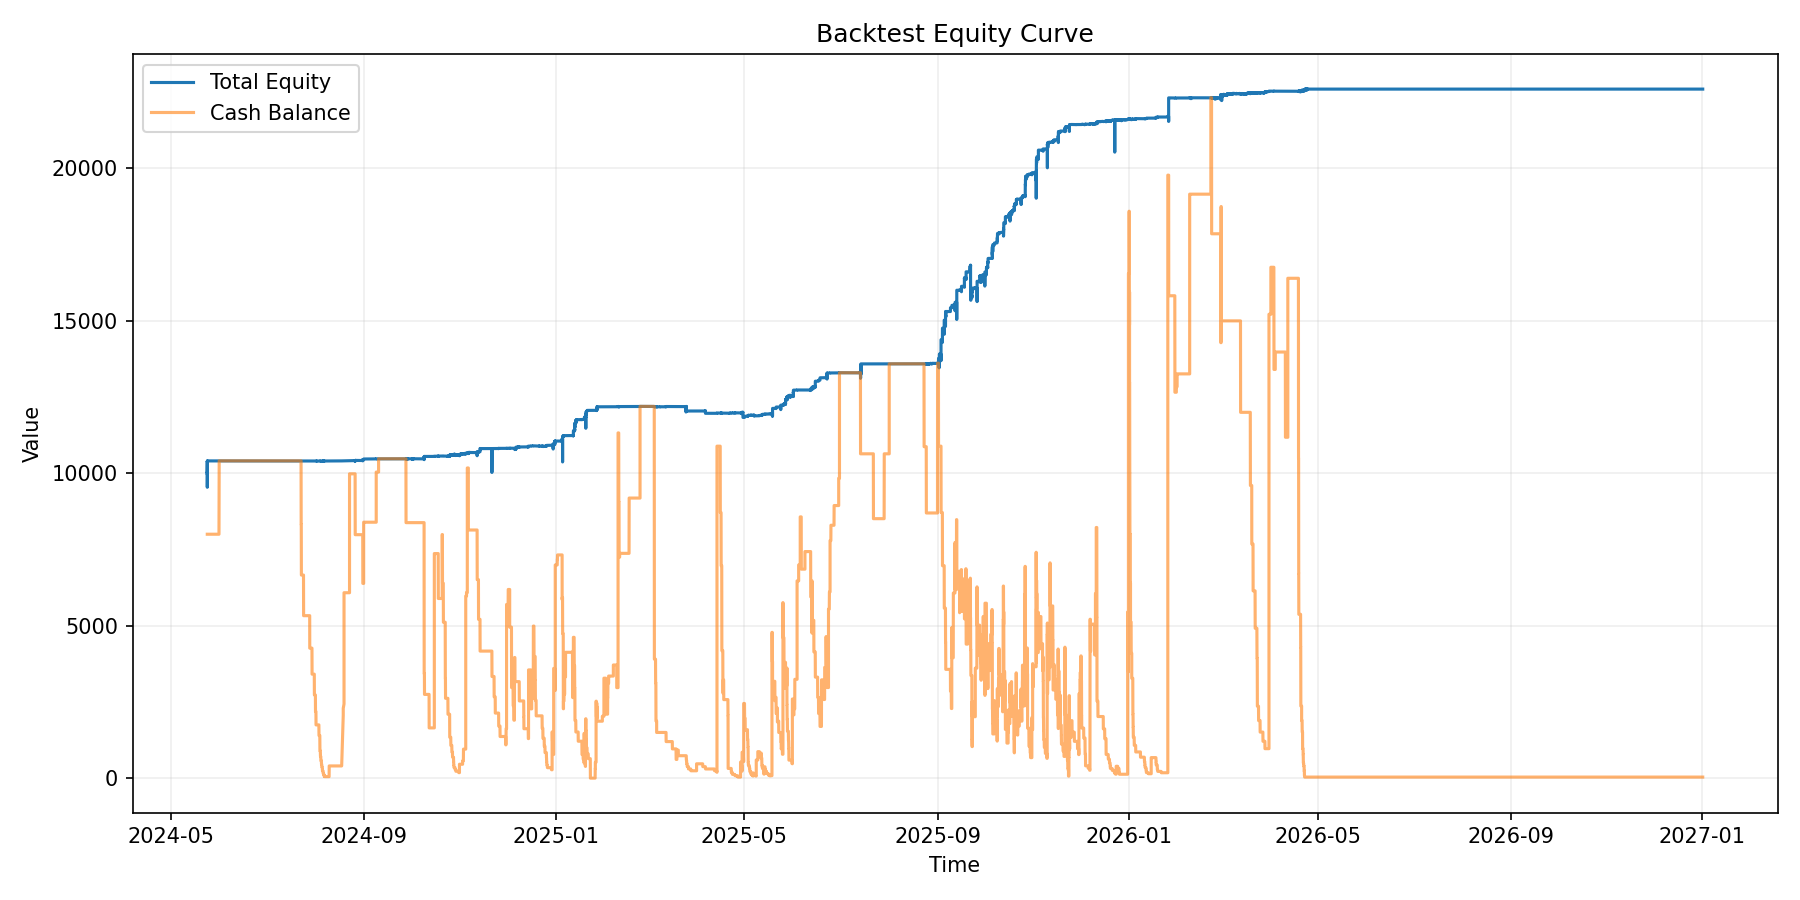
\includegraphics[width=0.92\linewidth]{figures/equity_curve.png}
  \end{center}
\end{frame}

\begin{frame}{Result Interpretation}
  \begin{itemize}
    \item High win rate comes from trading high-probability stable outcomes.
    \item Positive total equity indicates that the expert-following filter adds value over this sample.
    \item Final cash balance can be low because stable bucket sizing deploys substantial capital into open positions.
    \item The important portfolio value metric is total equity, not cash alone.
  \end{itemize}
\end{frame}

\begin{frame}{Main Risks and Limitations}
  \begin{itemize}
    \item Public API data may be incomplete or schema-shifting.
    \item Backtest assumes fills at delayed observed trade prices plus slippage.
    \item Liquidity and market impact are simplified.
    \item Open positions are marked using last known trade prices.
    \item Trader skill scores may overstate noisy small-sample performance.
    \item Parameter choices were research-driven and require out-of-sample validation.
  \end{itemize}
\end{frame}

\begin{frame}{Implemented but Disabled}
  The codebase includes several research features that are currently turned off
  in the reported configuration:

  \vspace{0.2cm}
  \begin{itemize}
    \item Lottery bucket: trades with $0.1 \leq p \leq 0.5$, controlled by a small fixed lot size.
    \item Lottery exposure cap: maximum lottery exposure as a fraction of total capital.
    \item Dynamic entry price cap: stricter or looser maximum entry price based on consensus confidence.
    \item Minimum edge filter: requires consensus-implied edge over entry price.
    \item Alternative trader-skill weighting: configurable historical notional exponent.
    \item Hashing-vectorizer embeddings: fast fallback for parameter sweeps.
  \end{itemize}
\end{frame}

\begin{frame}
  \centering
  \Huge Thank You
\end{frame}

\end{document}
